\chapter{Вступ}

\epigraph{Присвячується Маші та Міші}{}

\section{Системна інженерія та верифікація}
Протягом історії обчислювальної техніки було створено різні класи та способи обчислень,
різні тоеорії та підходи до програмування таких систем, різні класи систем програмування.
Зараз уже стало зрозумілим, що інженіринг систем які не піддаються до верифікації
формальними методами не може бути застосований у галузях де вимоги до якості
особливо підвищені, як то космонавтика, енергетика та фінанси.

\paragraph{}
Об'єктом дослідження данної роботи є системи верифікації програмного забезпечення
та операційні системи яки виконують
обчислення в реальному часі, їх поєднання та побудова формальної системи для
унифікованого середовища, яке поєднує середовище виконання та систему верифікації у єдину систему мов.
Розрізняють наступні класи систем верифікації (систем доведення теорем, або пруверів):
1) автоматизовані системи, які зосереджені на максимальній автоматизації процесу доведення (Z3, HOL, Coq);
2) системи програмування з конвертацією доведених програм в довільні мови (Idris, F*, Coq);
3) логічні фреймворки зі спеціальними логічними мовами для верифікації інших мов (Twelf, TLA+, NuPRL).

\paragraph{}
Предметом дослідження такої системи мов є теорія типів, яка вивчає обчислювальні властивості мов.
Теорія типів виділилася в окрему науку Пером Мартіном-Льофом як запит на вакантне місце у
трикутнику теорій, які відповідають ізоморфізму Каррі-Говарда-Ламбека (Логіки, Мови, Категорії).
Інші дві це: теорія категорій та логіка вищих порядків. Сама система доведення теорем є
логікою. Імплементація мови програмування,
яка релізує логічну семантику здійснюється завдяки теорії типів. Формалізація методів
відбувається завдяки теорії категорій, яка є абстрактною алгеброю фунцій,
метематичним інструментом для формалізації мов програмування та довільних
математичних теорій які описуються логіками вищих порядків.

\section{Історія систем верифікації}

\paragraph{}
Перші спроби пошуку формального фундаменту для теорії обчислень були покладені
Алонзо Черчем та Хаскелем Каррі у 30-х роках 20-го століття. Було запропоноване
лямбда числення як апарат який може замінити класичну теорію множин та її аксіоматику,
пропонуючи при цьому обчислювальну семантику. Пізніше в 1958, ця мова була втілена
у вигляді LISP лауреатом премії тюрінга Джоном МакКарті, який працював в Прінстоні.
Ця мова була побудована на конструктивних примітивах, які пізніше виявилися компонентами
індуктивних конструкцій та були формалізовані за допомогою
теорії категорій Вільяма Лавіра. Окрім LISP, нетипізоване лямбда числення
маніфестується у такі мови як Erlang, JavaScript, Python.
До цих пір нетипізоване лямбла числення є одною з мов у які робиться
конвертація доведених программ (екстракція).

\paragraph{}
Перший математичний прувер AUTOMATH (і його модифікації AUT-68 та AUT-QE),
який був написаний для комп'ютерів розроблявся під керівництвом де Брейна, 1967.
У цьому прувері був квантор загальності та лямбда функція, таким чином це був перший прувер
побудрваний на засадах ізоморфізма Каррі-Говарда-Ламбека.

\paragraph{}
ML/LCF або метамова і логіка обчисльювальних функцій був наступник крок до
осягнення фундаментальної мови простору, тут впреше з'явилися алебраїчні типи даних
у вигляді індуктивних типів, поліноміальних функторів або терміновані (well-founded) дерев.
Роберт Мілнер, асистований Морісом та Н'юві розробив Метамову (ML), як
інструмент для побудови прувера LCF. LCF був основоположником у родині пруверів
HOL88, HOL90, HOL98 та останньої версії на даний час HOL/Isabell.
Пізніше були побувані категорні моделі Татсоя Хагіно (CPL, Японія)
то Робін Кокетом (Charity, Канада).

\paragraph{}
У 80-90 роках були створені інші системи автоматичного доведення теорем,
такі як Mizar (Трибулєк, 1989). PVS (Оур, Рушбі, Шанкар, 1995),
ACL2 на базі Common Lisp (Боєр, Кауфман, Мур, 1996), Otter (МакКюн, 1996).

\newpage
\section{Методи верифікації}

\paragraph{}
Можна виділити два підходи до верифікації. Перший застосовується де вже є
певна програма написана на певній мові програмування і потрібно довести ізоморфність
цієї програми до доведеної моделі. Ця задача вирішується у побудові теоретичної моделі
для певної мови програмування, потім програма на цій мові переводиться у цю
теоретичну модель і доводить ізоморфізм цієї програми у побудованій моделі до доведеної моделі.
Приклади таких систем та піходів. VST (CompCert, сертифікація C програм),
NuPRL (Cornell University, розподілені системи, залежні типи),
TLA+ (Microsoft Reseach, Леслі Лампорт), Twelf (для верифікації мов програмування).

\paragraph{}
Інший підхід можна назвати підходом вбудованих DSL. Усе моделювання відбувається
в основній мові, а сертифіковані програми автоматично екстрагуються в довільні мови.
Приклади таких систем: Coq побудована на мові OCaml від науково-дослідного
інституту Франції INRIA; Agda побудовані на мові Haskell від шведського інституту технологій Чалмерс;
Lean побудована на мові C++ від Microsoft Research та Універсистету Каргені-Мелона;
Idris подудована на мові Haskell Едвіна Бреді з шотландського Університету ім. св. Андрія;
F* -- окремий проект Microsoft Research.

\paragraph{}
Завдання цього дослідження є побудова єдиної системи, яка поєднує середовище
викодання та систему верифікації програмного забезпечення. Це прикладне дослідження,
яке є сплавом фундаментальної математики та інженерних систем з формальними методами верицікації.

\newpage
\section{Метематичне забезпечення}
\vspace{0.3cm}

\subsection{Інтуіціоністична теорія типів Мартіна-Льофа}
Пер Мартін-Льоф в 1972 році запропонував $\Pi$, $\Sigma$ та $Id$
у якості основних фундаментальних типів. З тих пір усі сучасні системи типів
для пруверів побувані наслідуючи цю модель (MLTT, теорія типів Мартіна-Льофа).
Було показано, що мова такої системи
типів є внутрішнією мовою локальних декартово-замкнених категорій. $\Pi$ та $\Sigma$
кодують безпосереднь логічні кванторти $\forall$ та $\exists$, а тип $\rightarrow$ є
частковим випадком $\Pi$-типу, коли вираз $B$ не залежить від $x$.

\paragraph{}
Аксіоми:
\begin{equation}
\tag{$\Pi$}
\dfrac{\Gamma\ x:A \vdash B : Type\ \ \ \Gamma\ \vdash A : Type}
      {\Gamma\ \vdash \Pi (x : A) \rightarrow B (x) : Type}
\end{equation}

\begin{equation}
\tag{$\Sigma$}
\dfrac{\Gamma\ x:A \vdash B : Type\ \ \ \Gamma\ \vdash A : Type}
      {\Gamma\ \vdash \Sigma (x : A) \times B (x) : Type}
\end{equation}

\begin{equation}
\tag{$Id$}
\dfrac{\Gamma\ \vdash a: A\ \ \ \ \Gamma\ \vdash b: A\ \ \ \ \Gamma\ \vdash A : Type }
      {\Gamma\ \vdash Id_A (a,b)}
\end{equation}

Теореми:
\begin{center}
\begin{tabular}{lll}
  рефлексивність &:& $Id_A(a,a)$ \\
  підстановка    &:& $Id_A(a,a') \rightarrow B(x=a) \rightarrow B(x=a')$ \\
  симетричність  &:& $Id_A(a,b) \rightarrow Id_A(b,a)$  \\
  транзитивність &:& $Id_A(a,b) \rightarrow Id_A(b,c) \rightarrow Id_A(a,c)$ \\
  конгруентність &:& $(f: A \rightarrow B) \rightarrow Id_A(x,x') \rightarrow Id_B(f(x),f(x'))$ \\
\end{tabular}
\end{center}


\newpage
\subsection{Теорія категорій}

\paragraph{}
Теорія категорій широко застосовується як інструмент для математиків у тому числі і
при аналізі програмного забезпечення. Теорію категорій можна вважати абстрактною алгеброю функцій.
Дамо конструктивне визначення категорії.
Категорії (програми) визначаються переліком своїх об’єктів (типів) та своїх
морфізмів (функцій), а також бінарною операцією композиції,
що задовольняє закону асоціативності, та з тотожнім морфізмом (тотжньою функцією --- одиницею) який існує
для кожного об’єкту (типу) категорії. Аксіоми формації об’єктів не
приводяться та авто-постулуються в нижніх аксіомах.
Поки що тут буде визначатися тільки композиція морфізмів. Об’єкти $A$ та $B$ морфізма $f: A \rightarrow B$
називаються домен та кодомен відповідно. Композиція є фундаментальною властивістю морфізмів.

\paragraph{}
Інтро аксіоми -- асоціативність композиції та права і ліва композиції одниці показують,
що категорії є типизованими моноїдами, що складаються з морфізмів та операції композиції.
Є різні мови, у тому числі і графічні, представлення категорної семантики, однак у цій роботі
ми будемо використовувати теоретико-логічні формулювання.

\paragraph{}
Аксіоми:
\vspace{-0.5cm}
\begin{fullwidth}[width=\linewidth+3cm]
\hspace{-2cm}
\parbox[t][][l]{0.60\textwidth}{
\begin{prooftree}
\AxiomC{$\Gamma\ \vdash f: A \rightarrow B$ }
\AxiomC{$\Gamma\ \vdash g: B \rightarrow C$ }
\BinaryInfC{$\Gamma \vdash g \circ f : A \rightarrow C $}
\end{prooftree}

\begin{prooftree}
\AxiomC{$\Gamma \vdash f : B \rightarrow A$ }
\AxiomC{$\Gamma \vdash g : C \rightarrow B$ }
\AxiomC{$\Gamma \vdash h : D \rightarrow C$ }
\TrinaryInfC{$\Gamma \vdash (f \circ g) \circ h = f \circ (g \circ h) : D \rightarrow A $}
\end{prooftree}

}
\hspace{0.1cm}
\parbox[t][][r]{0.40\textwidth}{

\begin{prooftree}
\AxiomC{$$ }
\UnaryInfC{$\Gamma \vdash id_A : A \rightarrow A $}
\end{prooftree}

\begin{prooftree}
\AxiomC{$\Gamma\ \vdash f: A \rightarrow B$ }
\UnaryInfC{$\Gamma \vdash f \circ id_A = f : A \rightarrow B$}
\end{prooftree}

\begin{prooftree}
\AxiomC{$\Gamma\ \vdash f: A \rightarrow B$ }
\UnaryInfC{$\Gamma \vdash id_B \circ f = f : A \rightarrow B $}
\end{prooftree}

}

\end{fullwidth}
%Теореми:
%\begin{center}
%$(f \circ g) \circ h = f \circ (g \circ h)$\\
%$A \implies id : A \rightarrow A$\\
%$f \circ id = f$\\
%$id \circ f = f$\\
%\end{center}

\newpage
\subsection{Алгебраїчні типи даних}

Після операції композиції, як способу конструювання нових об’єктів
за допомогою морфізмів далі йде операція конструювання добутка двох об’єктів певної категорії,
разом з добутком морфізмів зі спільним доменом, необхідних для визначення декартового добутка $A \times B$.

\paragraph{}
Це є внутрішня мова декартової категорії, у якій для будь яких двох доменів існує їх декартова сума (кодобутку)
та декартовий добуток (косума, кортеж), за допомогою яких конструюються суми-протоколи та добутки-повідмоення,
а також існує $\bot$ тип-термінал, та $\top$ тип-котермінал. Термінальними типами зручно термінувати рекурсивні
типи даних, такі як списки. Ми будемо розглядати тільки категорії які маються добутки та суми.

\paragraph{}
Добуток має природні елімінатори $\pi$ зі спільним доменом, які є морфізмами-проекціями об’єктів добутка. Сума має оберненені
елімінатори $\sigma$ зі спільним кодоменом. Як видно добуток є дуальний до суми з точністю до направлення стрілок,
таким чином елімінатори $\pi$ та $\sigma$ є оберненими, тобто $\pi \circ \sigma = \sigma \circ \pi = id$.

\paragraph{}
Аксіоми:
\vspace{-0.5cm}
\begin{fullwidth}[width=\linewidth+2cm]
\hspace{-0.5cm}
\parbox[t][][l]{0.50\textwidth}{

\begin{prooftree}
\AxiomC{$\Gamma \vdash\ f:A \rightarrow B$ }
\AxiomC{$\Gamma \vdash\ g:A \rightarrow C$ }
\AxiomC{$\Gamma \vdash\ B \times C$ }
\TrinaryInfC{$\Gamma \vdash\ \langle f,g \rangle : A \rightarrow B \times C$ }
\end{prooftree}

\begin{prooftree}
\AxiomC{$\Gamma\ x: A \times B$ }
\UnaryInfC{$\Gamma \vdash \pi_1\ : A \times B \rightarrow A$;
           $\Gamma \vdash \pi_2\ : A \times B \rightarrow B$}
\end{prooftree}

\begin{prooftree}
\AxiomC{$\Gamma \vdash\  a:A$ }
\AxiomC{$\Gamma \vdash\  b:B$ }
\BinaryInfC{$\Gamma \vdash\ (a,b) : A \times B$ }
\end{prooftree}

\begin{prooftree}
\AxiomC{}
\UnaryInfC{$\Gamma \vdash\ \bot$ }
\end{prooftree}

}
\hspace{0cm}
\parbox[t][][r]{0.50\textwidth}{

\begin{prooftree}
\AxiomC{}
\UnaryInfC{$\Gamma \vdash\ \top$ }
\end{prooftree}

\begin{prooftree}
\AxiomC{$\Gamma \vdash\ a:A$ }
\AxiomC{$\Gamma \vdash\ b:B$ }
\BinaryInfC{$\Gamma\vdash a\ |\ b : A + B$}
\end{prooftree}

\begin{prooftree}
\AxiomC{$\Gamma\ x: A + B$ }
\UnaryInfC{$\Gamma \vdash \sigma_1: A \rightarrow A + B$;
           $\Gamma \vdash \sigma_2: B \rightarrow A + B$}
\end{prooftree}

\begin{prooftree}
\AxiomC{$\Gamma \vdash\ f:A \rightarrow B$ }
\AxiomC{$\Gamma \vdash\ g:A \rightarrow C$ }
\AxiomC{$\Gamma \vdash\ B + C$ }
\TrinaryInfC{$\Gamma \vdash\ [f,g] : A \rightarrow B + C$ }
\end{prooftree}
}
\end{fullwidth}
    Теореми:
\begin{fullwidth}[width=\linewidth+2cm]
\parbox[t][][l]{0.5\textwidth}{
$(f \circ g) \circ h = f \circ (g \circ h)$\\
$f \circ id = f$\\
$id \circ f = f$\\
$\pi_1 \circ \langle f, g \rangle = f$
}
%\hspace{-3cm}
\vspace{-1cm}
\parbox[t][][r]{0.4\textwidth}{
$\pi_2 \circ \langle f, g \rangle = g$\\
$\langle f \circ \pi_1, f \circ \pi_2 \rangle = f$\\
$\langle f, g \rangle \circ h = \langle f \circ h, g \circ h \rangle$\\
$\langle \pi_1, \pi_2 \rangle = id$
}
\end{fullwidth}

\newpage

\subsection{Лямбда числення}
Будучи внутрішньою мовою декартово-замкненої категорії лямбда числення окрім змінних
та констант у вигляді термів пропонує операції абстракції та аплікації, що визначає
достатньо лаконічну та потужну структуру обчислень з функціями вищих порядків,
та метатипизаціями, такими як System F, яка була запропонована
вперше Робіном Мілнером в мові ML, та зараз присутня в більш складних типоих системах,
таких як System F$\omega$, та системах Haskell та Scala.

\paragraph{}
З категоріальнї точки зору експоненти $f : A^B$ є аналогами
фукціональних просторів $f: B \rightarrow A$.
Так як ми вже визначили добутки та термінали, то ми можемо визначити і експоненти,
опускаючи усі категоріальні подробиці ми визначимо конструювання функції (операція абстракції),
яка параметризується змінною $x$ у середовищі $\Gamma$; та її елімінатора -- операції аплікації
функції до аргументу. Так визначаєьтся декартово-замкнена категорія.
Визначається також рекурсивний механізм виклику функції
з довільною кількістю аргументів.


\begin{fullwidth}
\hspace{-2cm}
\begingroup
\parbox[t][][l]{0.40\textwidth}{

Аксіоми:

\begin{prooftree}
\AxiomC{$\Gamma\ x:A \vdash M : B$}
\UnaryInfC{$\Gamma \vdash \lambda\ x\ .\ M : A \rightarrow B$}
\end{prooftree}

\begin{prooftree}
\AxiomC{$\Gamma\ f:A \rightarrow B$ }
\AxiomC{$\Gamma\ a:A$ }
\BinaryInfC{$\Gamma \vdash apply\ f\ a\ : (A \rightarrow B) \times A \rightarrow B$}
\end{prooftree}

\begin{prooftree}
\AxiomC{$\Gamma \vdash f: A \times B \rightarrow C$ }
\UnaryInfC{$\Gamma \vdash curry\ f : A \rightarrow (B \rightarrow C)$}
\end{prooftree}

}
\hspace{1cm}
\parbox[t][][r]{0.60\textwidth}{

Теореми:

\begin{center}
$apply \circ \langle (curry\ f) \circ \pi_1 , \pi_2 \rangle = f$\\
$curry\ apply \circ \langle g \circ \pi_1, \pi_2 \rangle) = g$\\
$apply \circ \langle curry\ f, g \rangle = f \circ \langle id , g\rangle$\\
$(curry\ f) \circ g = curry\ (f \circ \langle g \circ \pi_1,\pi_2\rangle)$\\
$curry\ apply = id$\\
\end{center}
}
\endgroup
\end{fullwidth}

\begin{center}
Об’єкти : $\top$\ |\ $\bot\ |\ \rightarrow\ |\ \times\ |\ +$\\
Морфізми : $id\ |\ f \circ g\ |\ [f,g]\ |\ \langle f, g \rangle\ |\ apply\ |\ \lambda\ |\ curry$
\end{center}

\newpage
\subsection{Індуктивні типи}
Системи з залежними типами як верифікаційні математичні формальні моделі
для доведення корректності. Система $\Sigma$ та $\Pi$ типів, як кванторів
існування та узагальнення. Системи Mizar, Coq, Agda, Idris, F*, Lean. Ми будемо
використовувати cubicaltt, Coq та Lean для доведення MLTT моделей.

\paragraph{}
Розбудовуючи певний фреймворк чи систему конструктивними методами
так чи інакше доведеться зробити певний вибір у мові та способі кодування.
Так при розробці теорії абстрактної алгебри в Coq були використані
поліморфні індуктивні структури. Однак Agda та Idris використувують
для побудови алгебраїчної теорії типи класів, а у Idris взагалі відсутні
поліморфірні індуктивні структури та коіндуктивні структури. В Lean
теж відсутні коіндуктивні структури проте повністю реалізована теорія
HoTT на нерекурсивних поліморфних структурах що обєднує основні чотири
класи математичних теорій: логіка, топологія, теорія множин, теорія типів.
Як було показано Стефаном Касом, одна з стратегій імплементації типів
класів --- це використання поліморфних структур.

\begin{equation}
\tag{$W$-formation}
\dfrac{A:Type\ \ \ \ x:A\ \ \ \ B(x):Type}
      {W (x:A) \rightarrow B(x) : Type}
\end{equation}

\begin{equation}
\tag{$W$-intro}
\dfrac{a:A\ \ \ \ t: B(a) \rightarrow W}
      {sup(a,t) : W}
\end{equation}

\begin{equation}
\tag{$W$-elimination}
\dfrac{w: W \vdash C(w) : Type\ \ \ \ x:A,\ u:B(x) \rightarrow W,\ \ \ \ v:\Pi (y:B(x)) \rightarrow C(u(y)) \vdash c(x,u,v):C(sup(x,u))}
      {w:W \vdash wrec(w,c):C(w)}
\end{equation}

\newpage
    \subsection{Числення процесів}
    Теорія $\pi$-числення процесів Роберта Мілнера є основним формалізмом обчислювальної
    теорії розподілених систем та її імплементації. З часів виникнення CSP числення розробленого Хоаром,
    Мілнеру вдалося значно розширити та адаптувати теорію до сучасних
    телекомунікаційних вимог, як наприклад хендовери в мобільних мережах.
    Основні теорми в моделі $\pi$-числення стосуються непротиречивості та неблокованості
    у синхронному виконанні мобільних процесів. Так як сучасний Web можно розглядати
    як телекомунікаційну систему, тому у розробці додатків можна покладатися у тому
    числі і на такі моделі як $\pi$-числення.
    Також ми анонсуємо процес як фундаменльний тип даних, подібний до функції але який здатний
    тримати певний стан у вигляді типа коротежа та є морфізмом-одиницею типу свого стану.

\begin{prooftree}
\AxiomC{$\Gamma\ \vdash E, \Sigma, X$ }
\AxiomC{$\Gamma\ \vdash action : \Sigma \times X \rightarrow \Sigma \times X$ }
\BinaryInfC{$\Gamma \vdash {spawn}\ action : \pi_\Sigma $}
\end{prooftree}

\begin{prooftree}
\AxiomC{$\Gamma\ \vdash pid : \pi_\Sigma$ }
\AxiomC{$\Gamma\ \vdash msg : \Sigma$ }
\BinaryInfC{$\Gamma \vdash join\ msg\ pid : \Sigma \times \pi_\Sigma \xrightarrow{\bullet} \Sigma$;
            $\Gamma \vdash send\ msg\ pid : \Sigma \times \pi_\Sigma \rightarrow \Sigma$}
\end{prooftree}

\begin{prooftree}
\AxiomC{$\Gamma\ \vdash L : A + B, R : X + Y$ }
\AxiomC{$\Gamma\ \vdash M : A \rightarrow X, N : B \rightarrow Y$ }
\BinaryInfC{$\Gamma \vdash receive\ L\ M\ N : L \xrightarrow{\bullet} R$}
\end{prooftree}
\paragraph{}

    \paragraph{}
    Алгебра процесів визначає базові операції мультиплексування двох чи декількох
    протоколів в рамках одного процесу (добуток), а також паралельного запуску процесів (сума).

\begin{center}
\begin{tabular}{lcl}
$\oplus$   &:& $\pi \parallel \pi$\\
$\otimes$  &:& $\pi \mid \pi$\\
\end{tabular}
\end{center}

\newpage
\section{Дослідження систем типів}
Головна ідея цієї роботи -- побудова гнучкої сучасної мови,
яка здатна була би обслуговувати академію та виробництво,
тобто у якій можно було би створювати моделі, тут же у цій мові їх доводити,
та екстрагувати код через оптимізоване ядро у інтерпритатор чи мови які продукують машинний код.

\paragraph{}
Працюючи над розподіленими системами, системами зберігання даних та
системами обробки тензорних масивів, автором було виявлено глибокий
зв'язок Pi-числення процесів (Erlang, Ling) і Stream-числення для обробки
тензорних масивів (Futhark, Spiral). Тому ми почали займатися дослідженням
гнучкої типової системи яка би могла поєднувати різні моделі мов з одним
уніфокованим MLTT ядром.

\paragraph{}
В ході дослідження були виявлені основні типові системи, або мовні рівні, які
пропонується сприймати як протоколи, які можуть підключатися додаючи до
системи нові мовні рівні.

\subsection{PTS системи}
З тих часів, як Кокуанд відкрив числення конструкцій, та Берендрехт систематизував його варіації,
теорія чистих типових систем (Pure Type Systems, PTS) стала вже достатньо розробленою.
Також вона відома як теорія з одніє аксіомою --- $\Pi$-типом MLTT теорії без $\Sigma$ та $Id$ типа. Ця теорія репрезентую функціональну повноту
згідно Герміди-Якобса.

\begin{lstlisting}[mathescape=true]
name: U = list nat

data $O_1$ = star (n: nat)
         | var (n: name)
         | app (f a: $O_1$)
         | lambda (x: name) (d c: $O_1$)
         | arrow (d c: $O_1$)
         | pi (x: name) (d c: $O_1$)
\end{lstlisting}

Такі системи є простими, проте зрозумілими та досить потужними, аби реалізувати на такій системі
системі $System F$ бібліотеку. Нами була вибрана система $PTS_{\infty}$,
яка підтримує нескінченну кількість всесвітів, що унеможливлює парадокси Хуркенса-Рассела-Жирара
і має два режими: предикативний та імпредикативний. Ця система типів представлена
у нашій роботі як мова $Om$, яка виступає ядром системи доведення, верифікації та екстрагування.

\newpage
\subsection{MLTT системи}
Для доведення теорем необхіден $\Sigma$-тип, а також рівність на твердженнях.
Саме тому теорія типів Мартіна-Льофа з самого початку була облаштова цими конструціями.
В MLTT $\Sigma$-тип репрезентує контекстуальну повноту згідно Герміди-Якобса.
$\Sigma$-тип необхідний також для моделювання алгебраїчних структур-носіїв.

\begin{lstlisting}[mathescape=true]
data $O_2$ = $O_1$
         | sigma (n: name) (a b: $O_2$)
         | pair (a b: $O_2$)
         | fst (p: $O_2$)
         | snd (p: $O_2$)

data $O_3$ = $O_2$
         | id (a b: $O_3$)
         | idPair (a b: $O_3$)
         | idJ (a b c d e: $O_3$)
\end{lstlisting}

\subsection{Індуктивні системи}
В процесі глибшого дослідження індукції в MLTT теорії виникла теорія індуктивних типів,
поліноміальних функторів у застосуванні до теорії типів (або рекурсивних дерев
з визначеною базою рекурсії, W-типи). В мовах програмування вони відомі як data типи.
Насправді індуктивні типи можуть бути закодовані в PTS системах за допомогою
кодування Черча-Бома-Берардуччі, або в інших системах кодувань (Парігот, Скот, CPS, Ламбек).
Рекурсивні дерева без бази рекурсії називаються ко-індуктивними типами, та
часто можуть бути представлені як record типи, або рекурсивні record типи.

\begin{lstlisting}[mathescape=true]
data tele   (A: U) = nil | tel (n: name) (b: A) (xs: tele A)
data branch (A: U) =        br (n: name) (a: list name) (t: A)
data label  (A: U) =       lab (n: name) (t: tele A)

data $O_4$ = $O_3$
         | sum  (n: name) (t: tele $O_4$) (labels:      list (label $O_4$))
         | case (n: name) (t: ind)      (branches: list (branch $O_4$))
         | ctor (n: name)               (args:     list $O_4$)
\end{lstlisting}

\newpage
\subsection{HTS системи}
Багаточисельні фундаменальні дослідження рівності в MLTT теорії привели
до тактування $\infinity-групоїдів$ як топологічних просторів. Так в чекарах
виник $Path$-тип, розширений багатовимірний варінт $Id$-типу з оригінальної теорії Мартіна-Льофа.
Це тип моделює відрізок $[0,1]$ разом з алгеброю де Морана на цьому інтервалі.
Ця система типів необхідна для доведення гомотопічних теорем та при роботі з
вищими індуктивними типами, за домогою яких кодуються топологічні об'єкти:
багатовимірник відрізок, багатовимірна сфера, топологічні операції.
Такі системи типів називаються гомотопічними (Homotopy Type System, HTS)
та вперше були запропоновані Воєводським.

\begin{lstlisting}[mathescape=true]
data alg = zero
         | one
         | max (a b: alg)
         | min (a b: alg)

data $O_5$ = $O_4$
         | path (a b: $O_5$)
         | pathLam (n: name) (a b: $O_5$)
         | pathApp (f: alg) (a b: $O_5$)
         | comp (a b: $O_5$)
         | fill (a b c: $O_5$)
         | glue (a b c: $O_5$)
         | glueElem (a b: $O_5$)
         | unglueElem (a b: $O_5$)
\end{lstlisting}

\subsection{Pi-числення}

\subsection{Числення алгебраїчних ефектів}

\subsection{Обробка тензорних масивів}

\newpage
\section{Дослідження середовищ виконання}

Усі середовища виконання можно умовно розділити на два класи:
1) інтерпретатори нетипізованого або просто
типізованого (рідше з більш потужними системами типів),
лямбда числення з можливими JIT оптимізаціями; та 2)
безпосередня генерація інструкцій процессора і лінкування цієї програми з
середовищем виконання що забезпечує планування ресурсів
(в цій області переважно використовується System F типізація).

\paragraph{}
До першого класу можно віндеси такі віртуалні машини та інтерпретатори як
Erlang (BEAM), JavaScript (V8), Java (HotSpot), K (Kx), PHP (HHVM), Python (PyPy), LuaJIT
та багато інших інтерпретаторів.

\paragraph{}
До другого класу можна віднести такі мови програмування: ML, OCaml, Rust,
Haskell, Pony. Часто використовується LLVM як спосіб генерації програмного коду,
однак на момент публікації статті немає промислового верифікованого LLVM генератора.
Rust використовує проміжну мову MIR над LLVM рівнем. Побудова верифікованого компілятора
для такого класу систем виходить за межі цього дослідження. Нас тут буде цікавити
лише вибір найкращого кандидата для середовижа виконання.

\paragraph{}
Нійбільш цікаві цільові платформи для виконання программ
які побудовані на основі формальних доведень для нас є OCaml (тому,
що це основна мова естракту для промислової системи доведення теорем Coq),
Rust (тому, що рантайм може бути написаний без використання сміттєзбірника),
Erlang (тому, що підтримує неблоковану семантику пі-калкулуса)
та Pony (тому, що семантика його пі-калкулуса побудована на імутабельних чергах та CAS курсорах).
У цій роботі ми зосередимося на дослідженні тьох підходів
та побудові трьох прототипів.



\newpage
\section{Продукти дослідження}

\subsection{Інтерпретатор О на Rust для L4}
Перший прототип, рантайм О -- лінивий
векторизований інтерпретатор (підтримка SSE/AVX інструкцій) та система
управління ресурсами з планувальником лінивих програм
та системою черг і CAS курсорсів у якості моделі пі-калкулуса. Розглядається також
використання ядра L4 на мові С, верифікованого за допомогою HOL/Isabell,
у якості базової операційної системи.

\subsection{Коіндукція на Coq з екстрактом в OCaml}
Другий прототип побудований на базі coq.io, що дозволяє
використовувати бібліотеки OCaml для промислового програмування в Coq.
У цій роботі ми формально показали і продемонстрували коіндуктивний шел
та вічно працюючу тотальну програму на Coq. Ця робота проводилася
в рамках дослідження системи ефектів для результуючої мови програмування.

\subsection{Екстракція в Erlang та О з ОМ}
Третій прототип -- побудова тайпчекера та ектрактора у мову Erlang та O.
Ця робота представлена у вигляді PTS тайпчекера ОМ, який вистує у ролі
проміжної мови для повної нормалізації лямбда термів. В роботі використане
нерекурсивне кодування індуктивних типів та продемонстрована теж бескінечна
тотальна программа у якості способу лінкування з підсистемою вводу-виводу
віртуальної машини Erlang.

\subsection*{Idris та PureScript разом з Erlang}
Також був досліджений спосіб естракції Erlang програм з мови програмування
Idris, розглянутий протокол передачі термів-теорем в Lean,
та екстракція з PureScript в Erlang.


\newpage
\section{Структура роботи}

\begin{center}
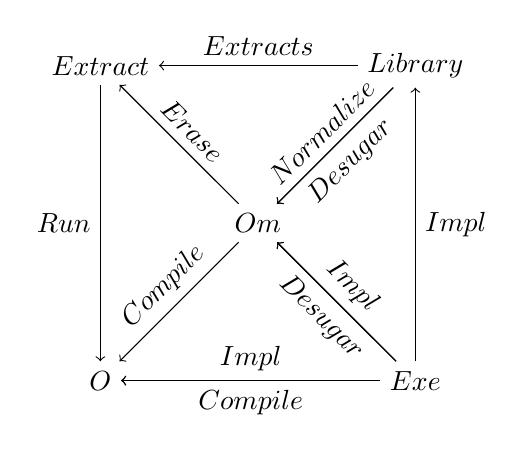
\begin{tikzpicture}
\tikzstyle{every initial by arrow}=[]
    \node (a) at (0,0) {$O$};
    \node (b) at (0,4) {$Extract$};
    \node (c) at (4,0) {$Exe$};
    \node (d) at (4,4) {$Library$};
    \node (e) at (2,2) {$Om$};
    \draw [->] (b) to node [left] {$Run$} (a);
    \draw [->] (c) to node [below] {$Compile$} (a);
    \draw [->] (c) to node [above] {$Impl$} (a);
    \draw [->] (e) to node [above,sloped] {$Compile$} (a);
    \draw [->] (d) to node [above,sloped] {$Normalize$} (e);
    \draw [->] (d) to node [below,sloped] {$Desugar$} (e);
    \draw [->] (d) to node [above] {$Extracts$} (b);
    \draw [->] (c) to node [right] {$Impl$} (d);
    \draw [->] (e) to node [above,sloped] {$Erase$} (b);
    \draw [->] (c) to node [below,sloped] {$Desugar$} (e);
    \draw [->] (c) to node [above,sloped] {$Impl$} (e);
\end{tikzpicture}
\end{center}

\begin{fullwidth}
\hspace{-2cm}
\begin{tabular}{lll}
  $Exe \xrightarrow{Impl} Om$ &---& На прувері пишеться ядро \\
  $Exe \xrightarrow{Impl} O$ &---& На прувері пишеться інтерпретатор \\
  $Exe \xrightarrow{Impl} Exe$ &---& Прувер написаний сам на собі \\
  $Exe \xrightarrow{Impl} Library$ &---& На прувері пишеться базова бібліотека \\
  $Exe \xrightarrow{Desugar} Om$ &---& Сам прувер є розширенням ядра \\
  $Library \xrightarrow{Desugar} Om$ &---& Базова бібліотека конвертується в код ядра \\
  $Library \xrightarrow{Normalize} Om$ &---& Повна нормалізація базової бібліотеки \\
  $Om \xrightarrow{Erase} Extract$ &---& Видаляється інформація про типи, детипізація \\
  $Extract \xrightarrow{Run} O$ &---& Запуск на інтерпритаторі \\
\end{tabular}
\end{fullwidth}
